
% VLDB template version of 2020-08-03 enhances the ACM template, version 1.7.0:
% https://www.acm.org/publications/proceedings-template
% The ACM Latex guide provides further information about the ACM template

\documentclass[sigconf, nonacm]{acmart}

%% The following content must be adapted for the final version
% paper-specific
\newcommand\vldbdoi{XX.XX/XXX.XX}
\newcommand\vldbpages{XXX-XXX}
% issue-specific
\newcommand\vldbvolume{14}
\newcommand\vldbissue{1}
\newcommand\vldbyear{2020}
% should be fine as it is
\newcommand\vldbauthors{\authors}
\newcommand\vldbtitle{\shorttitle} 
% leave empty if no availability url should be set
\newcommand\vldbavailabilityurl{URL_TO_YOUR_ARTIFACTS}
% whether page numbers should be shown or not, use 'plain' for review versions, 'empty' for camera ready
\newcommand\vldbpagestyle{plain} 

\begin{document}
\title{Replication of JSON schema discovery for JSON schema extraction}

%%
%% The "author" command and its associated commands are used to define the authors and their affiliations.
\author{Lutfi}
\affiliation{%
  \institution{University of Passau}
  \city{passau}
  \country{Germany}
}
\email{lutfi01@ads.uni-passau.de}
\email{lutfidman.19997@gmail.com}

%%
%% The abstract is a short summary of the work to be presented in the
%% article.

\maketitle


%%% do not modify the following VLDB block %%
%%% VLDB block start %%%
\ifdefempty{\vldbavailabilityurl}{}{
\vspace{.3cm}
\begingroup\small\noindent\raggedright\textbf{PVLDB Artifact Availability:}\\
The source code, data, and/or other artifacts have been made available at \url{https://github.com/lutfilutfi/JSONSchemaDiscovery}.
\endgroup
}
%%% VLDB block end %%%

\section{Introduction}
With the growing popularity of nosql database more documents are being stored in JSON files. And its important 
JSON schema discovery\cite{1} is a saas(software as a service) and is  a tool to extract JSON schema from JSON and BSON(extended JSON) files. We utilize a mean stack(Mongo Express Angular Node) to run the client and the server. We attempt to obtain JSON schema for the five documents as done in the paper \cite{1}. 
The tool works in a sequence of 4 steps :
\begin{enumerate}
\item 1.Document raw schema generation
\item 2.Grouping of document raw schemas
\item 3.Unification of document raw schemas
\item 4.JSON Schema generation.
\end{enumerate}
Schema extraction is possible from mongoDB collections(collections are analogicaly similar to a table in SQL database). In this replication package we aim to test if schema definations matches the one generated by experiments. We then verify it by running diff command

\section{JSON schema discovery tool}

Instructions on how to run the tool and verify the experiment is found in the readme of the repository. The entire stack (Angular, node, express, mongo) used is free and open source. Apache license 2.0 is used. Foursquare and DBPedia data sets were not used because former was paid for querying large dataset and DBpedia dataset did not return NJSON did not match while using SPARQL to query for rdfs.

\subsection{Hypothesis and replicating the experiment }

Our goal is to find if the JSONSchemaDiscovery app generates the schema defination accurately for the given extended json files. We need to confirm that the schema definition of the extended bson files to be the same as JSON schema in examples folder bsontypestestjsonschema. We need to use mongorestore to to create the collection using the .bson files. Then we extract schema and download the results.

\begin{figure}
  \centering
  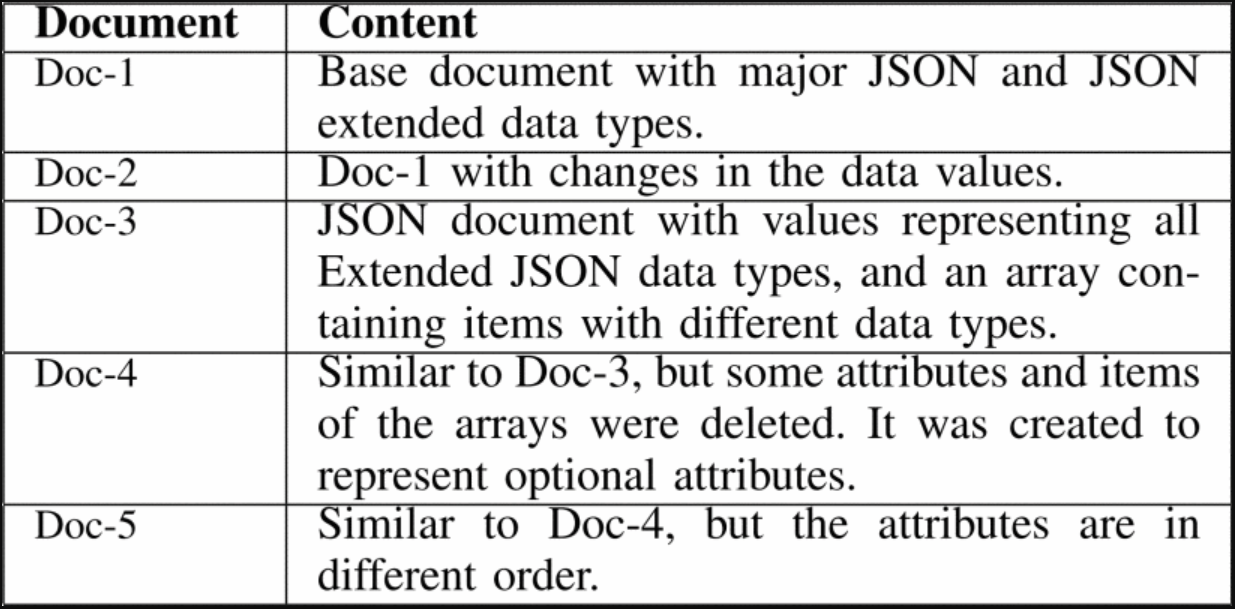
\includegraphics[width=\linewidth]{figures/figure1.PNG}
  \caption{Description of bson files}
  \label{fig:BSON}
\end{figure}

\begin{figure}
  \centering
  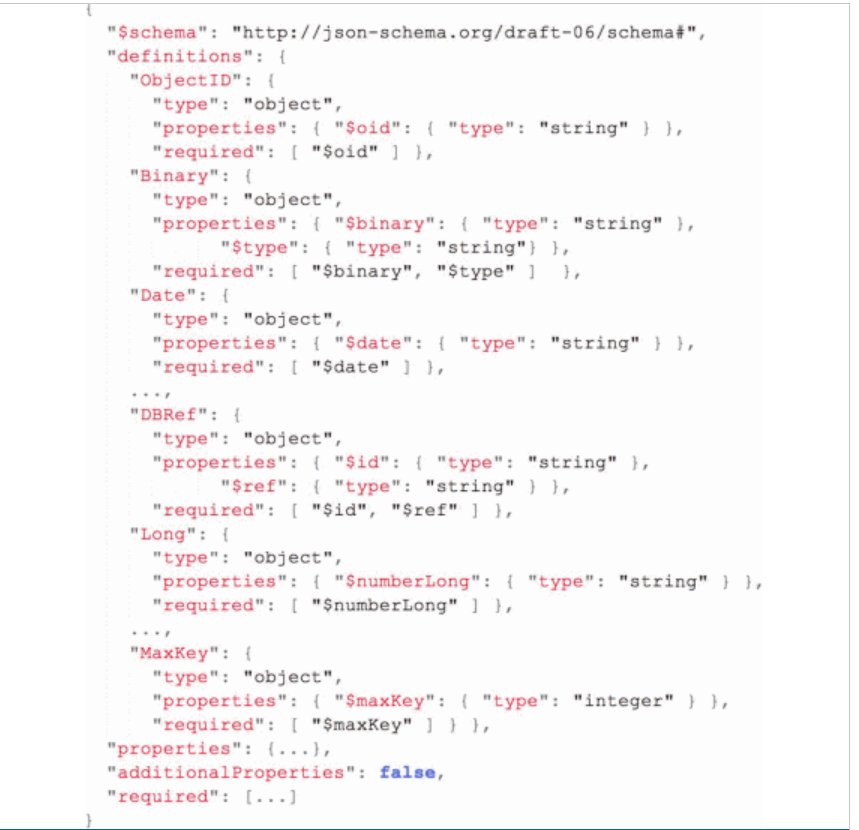
\includegraphics[width=\linewidth]{figures/figure2.PNG}
  \caption{Schema definition}
  \label{fig:schema definition}
\end{figure}


\subsection{Verification of Results}
 In order to verify the results, the schema definition must be downloaded from the application and checksimilar python script must be run with modification to file names

%\clearpage

\bibliographystyle{ACM-Reference-Format}
\bibliography{sample}

\end{document}
\endinput
